\documentclass[10pt]{article}

% ---------------------------------------------------------------- layout
\usepackage[letterpaper, textwidth=5.5in, textheight=9in, centering, headheight=14pt]{geometry}
\usepackage[T1]{fontenc}
\usepackage[utf8]{inputenc}
\usepackage{times}
\usepackage{mathptmx}
\usepackage{amsmath, amssymb, amsthm, bm}
\usepackage{booktabs, multirow, array}
\usepackage{graphicx}
\usepackage[dvipsnames]{xcolor}
\usepackage{tikz}
\usetikzlibrary{positioning, arrows.meta, calc}
\usepackage[round]{natbib}
\usepackage{microtype}
\usepackage{enumitem}
\usepackage[font=small, labelfont=bf]{caption}
\usepackage{algorithm}
\usepackage{algpseudocode}
\usepackage{xspace}
\usepackage{pifont}
\usepackage{fancyhdr}
\usepackage[section]{placeins}
\usepackage[colorlinks=true, linkcolor=MidnightBlue, citecolor=MidnightBlue, urlcolor=MidnightBlue]{hyperref}
\usepackage[capitalise, noabbrev]{cleveref}

% ---------------------------------------------------------------- macros
\newcommand{\cmark}{\textcolor{ForestGreen}{\ding{51}}}
\newcommand{\xmark}{\textcolor{BrickRed}{\ding{55}}}
\newcommand{\pmark}{\textcolor{Dandelion}{$\boldsymbol{\sim}$}}
\newcommand{\TBD}{\textcolor{red}{\textbf{[TBD]}}\xspace}
\newcommand{\todo}[1]{\textcolor{red}{[TODO: #1]}}
\newcommand{\ASK}{\textup{\textsc{ask}}\xspace}
\newcommand{\EXEC}{\textup{\textsc{exec}}\xspace}
\newcommand{\REFUSE}{\textup{\textsc{refuse}}\xspace}
\newcommand{\ADA}{AgentDojo-Ask\xspace}
\newcommand{\E}{\mathbb{E}}
\newcommand{\ind}{\mathbf{1}}
\newcommand{\dyn}{\mathrm{dyn}}
\DeclareMathOperator*{\argmax}{arg\,max}

\theoremstyle{plain}
\newtheorem{proposition}{Proposition}
\newtheorem{lemma}{Lemma}
\newtheorem{corollary}{Corollary}
\theoremstyle{definition}
\newtheorem{assumption}{Assumption}
\crefname{assumption}{Assumption}{Assumptions}
\crefname{proposition}{Proposition}{Propositions}
\crefname{lemma}{Lemma}{Lemmas}
\crefname{corollary}{Corollary}{Corollaries}
\crefname{algorithm}{Algorithm}{Algorithms}

\setlist{itemsep=1pt, topsep=3pt, parsep=0pt}

% numbers produced by sim/simulate.py
% Auto-generated by sim/simulate.py -- do not edit by hand.
\newcommand{\SimLdagger}{12.8}
\newcommand{\SimMuTenZero}{0.299}
\newcommand{\SimMuTenEight}{0.247}
\newcommand{\SimMuThirtyfiveEight}{0.069}
\newcommand{\SimSweepMinASR}{20.6}
\newcommand{\SimSweepMinAsks}{8.8}
\newcommand{\SimSweepMaxAsksASR}{48.3}
\newcommand{\SimSweepMaxAsks}{31.5}
\newcommand{\SimFloodStaticTwenty}{90}
\newcommand{\SimFloodStaticMax}{91}
\newcommand{\SimFloodDPMax}{2}
\newcommand{\SimFloodMyopicMax}{9}
\newcommand{\SimFloodDPDoneFifty}{17}
\newcommand{\SimPowerSmall}{15}
\newcommand{\SimPowerSmallTwenty}{10}
\newcommand{\SimPowerMedium}{10}
\newcommand{\SimPowerLarge}{5}
\newcommand{\SimAutoASR}{14.7}
\newcommand{\SimAutoBenign}{82.9}
\newcommand{\SimAutoAsks}{0.0}
\newcommand{\SimAutoReward}{23.9}
\newcommand{\SimAlwaysASR}{67.3}
\newcommand{\SimAlwaysBenign}{100.0}
\newcommand{\SimAlwaysAsks}{40.0}
\newcommand{\SimAlwaysReward}{1.0}
\newcommand{\SimStaticASR}{34.8}
\newcommand{\SimStaticBenign}{99.7}
\newcommand{\SimStaticAsks}{18.7}
\newcommand{\SimStaticReward}{18.2}
\newcommand{\SimMyopicASR}{9.6}
\newcommand{\SimMyopicBenign}{92.7}
\newcommand{\SimMyopicAsks}{11.6}
\newcommand{\SimMyopicReward}{27.2}
\newcommand{\SimDPASR}{10.5}
\newcommand{\SimDPBenign}{95.3}
\newcommand{\SimDPAsks}{9.0}
\newcommand{\SimDPReward}{28.3}
\newcommand{\SimOracleLambda}{28.7}
\newcommand{\SimOracleAsks}{10.3}
\newcommand{\SimOracleUtil}{28.7}
\newcommand{\SimLVanLambda}{174}
\newcommand{\SimLFixLambda}{29.9}
\newcommand{\SimLFixASR}{5.2}
\newcommand{\SimLFixAsks}{10.0}
\newcommand{\SimLFixUtil}{27.5}
\newcommand{\SimLFixRatio}{96}
\newcommand{\SimLRandASR}{5.1}
\newcommand{\SimLRandAsks}{11.1}
\newcommand{\SimLRandUtil}{27.3}
\newcommand{\SimLRandRatio}{95}
\newcommand{\SimLNofatASR}{52.9}
\newcommand{\SimLNofatAsks}{39.1}
\newcommand{\SimLNofatUtil}{28.1}
\newcommand{\SimLNofatRatio}{98}
\newcommand{\SimLVanASR}{25.7}
\newcommand{\SimLVanAsks}{5.1}
\newcommand{\SimLVanUtil}{34.7}
\newcommand{\SimLVanRatio}{121}
\newcommand{\SimNsessions}{20{,}000}
\newcommand{\SimIters}{2000}
\newcommand{\SimGenNofatWorstASR}{62}
\newcommand{\SimGenFixWorstASR}{10}
\newcommand{\SimGenRandWorstASR}{10}


\pagestyle{fancy}
\fancyhf{}
\fancyhead[C]{\footnotesize\textcolor{red!75!black}{DRAFT --- theory and stylized simulations are real; AgentDojo-Ask and user-study results are placeholders [TBD]}}
\fancyfoot[C]{\thepage}
\renewcommand{\headrulewidth}{0pt}

\title{\textbf{Asking Under Attack: Learning Fatigue-Aware\\Confirmation Policies for LLM Agents}}
\author{Hassan [Surname]\\ ENSICAEN, Caen, France\\ \texttt{[email]}}
\date{Working draft --- November 2026}

\begin{document}
\maketitle
\thispagestyle{fancy}

\begin{abstract}
Tool-using LLM agents increasingly pause to ask their users before consequential actions, and this confirmation is often the last defense against indirect prompt injection. Yet human attention is finite: each question spends some of the user's vigilance, and an attacker can exhaust it on purpose. We study \emph{when} an agent should ask. We model confirmation as a constrained POMDP in which the probability that the user catches a malicious request decays with the number of confirmations already requested. For one decision we derive a three-zone rule (execute, ask, refuse) whose ask band shrinks with the user's load and vanishes beyond a finite load $\ell^\dagger$. In the sequential problem each question carries a \emph{price of attention} that narrows the band further, so fatigue-aware but myopic guards provably over-ask; under a power-law ranking model the load that catches the most attacks is interior and keeps vigilance above one half. We then propose a GRPO-Lagrangian method that trains the agent's ask policy against simulated fatiguing users in \ADA, an extension of AgentDojo with effect-bound confirmations, multi-task sessions and attacks on the confirmation channel itself (flooding, suppression, disguise). Stylized simulations predict the shape of our main results: attack success is U-shaped in the asking rate; a policy trained against a never-tiring simulated user asks \SimLNofatAsks{} times per session and lets \SimLNofatASR\% of attacks through once users tire; and the per-group reward standardization of vanilla GRPO breaks the Lagrangian, while a batch-level scale approximately meets a 5\% attack budget with \SimLFixRatio\% of the optimal utility. The pilot user study and the \ADA experiments are in progress.
\end{abstract}

\begin{center}
\fcolorbox{red!70!black}{red!4}{\parbox{0.96\linewidth}{\small
\textbf{Status of this draft.} Sections~\ref{sec:problem}--\ref{sec:theory} (formulation, theory, proofs) and \S\ref{sec:sim} (stylized simulations) are complete; every number there comes from \texttt{sim/simulate.py}. Figures labeled \emph{stylized} are predictions of curve \emph{shapes}, not benchmark results. The pilot user study (\S\ref{sec:pilot}) and the \ADA experiments (\S\ref{sec:agentdojo}) are designed but not run: their results are marked \TBD and their tables contain ``--''. Citation entries marked TODO in \texttt{refs.bib} must be checked.}}
\end{center}

% ============================================================================
\section{Introduction}\label{sec:intro}

LLM agents now read email, move money and edit calendars through tools. This makes them vulnerable to \emph{indirect prompt injection}: instructions hidden in the data an agent reads---an email, a web page, a calendar invitation---can redirect its tool calls toward an attacker's goal \citep{greshake2023not}. Benchmarks such as AgentDojo and InjecAgent show that capable agents remain vulnerable \citep{debenedetti2024agentdojo,zhan2024injecagent}, and adaptive attacks bypass most published defenses \citep{nasr2025attacker,chen2026learning,autodojo2026}.

Because no defense is perfect, deployed agents keep a human in the loop: before a consequential action they pause and ask the user to confirm \citep{openai2025operator,kolluri2026prudentia,effectguard2026}. The user becomes the last line of defense. But this defense has a capacity. Usable-security research shows that people habituate to warnings and click through them \citep{akhawe2013alice,bravolillo2013attention,anderson2015polymorphic}; vigilance declines during sustained monitoring \citep{warm2008vigilance}; clinicians learn to ignore alarms that ring too often \citep{cvach2012alarm}. An agent that asks too often teaches its user to approve. An attacker who knows this can first trigger many harmless-looking requests and then slip the harmful one through \citep{turan2026oversight}.

This paper asks a simple question: \emph{when should a tool-using agent ask for confirmation, if each question spends user attention and an adversary may target the confirmation channel?} Work on asking usually treats the user as a reliable oracle with a fixed cost per question \citep{overman2026oversight,trinh2026hilbench,dossantos2026act,zhang2026askless}. Work on fatigue-aware deferral either does not consider tool-using agents and adversaries \citep{zhang2026falcon} or calibrates an external guard without learning the agent's own policy \citep{turan2026oversight}. We bring three ingredients together: a learned ask policy, a user whose vigilance depends on the agent's own past questions, and an attacker who targets both the agent and the confirmation channel (\Cref{fig:overview}). Our contributions are:
\begin{enumerate}[leftmargin=*]
\item \textbf{Formulation (\S\ref{sec:problem}).} We cast fatigue-aware confirmation as a constrained POMDP whose state includes the user's load $\ell_t$, with the attacker's influence as a hidden variable.
\item \textbf{Theory (\S\ref{sec:theory}).} We show (i) a three-zone rule whose ask band shrinks with load and vanishes at a finite load $\ell^\dagger$ (\Cref{prop:zones}); (ii) a \emph{price of attention} that narrows the band in the sequential problem, so that myopic guards over-ask (\Cref{prop:dynamic}, \Cref{cor:overask}); (iii) a closed-form optimal confirmation load under a power-law ranking model (\Cref{prop:load}).
\item \textbf{Environment and method (\S\ref{sec:method}).} We introduce \ADA, which adds an effect-bound \ASK action, simulated fatiguing users, multi-task sessions and three attacks on the confirmation channel to AgentDojo. We train the ask policy with a GRPO-Lagrangian algorithm, and show that GRPO's per-group standardization silently reweights the Lagrangian; a batch-level scale fixes it.
\item \textbf{Evidence (\S\ref{sec:pilot}, \S\ref{sec:results}).} Stylized simulations predict the shape of every main result, and a pilot user-study protocol with a simulated power analysis will calibrate the fatigue model. \ADA results are in progress (\TBD).
\end{enumerate}

\begin{figure}[t]
\centering
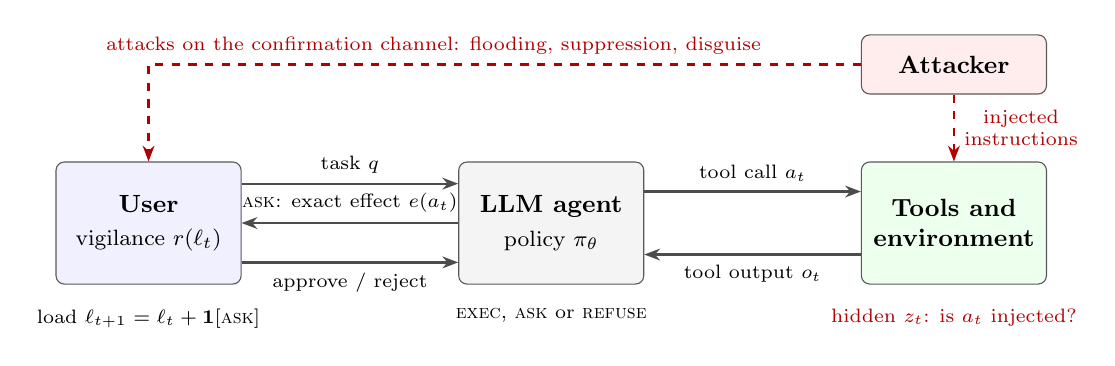
\begin{tikzpicture}[
  font=\small,
  box/.style={draw=black!65, rounded corners=3pt, minimum width=2.35cm, minimum height=1.55cm, align=center, fill=#1},
  box/.default=white,
  arr/.style={-{Stealth[length=2mm]}, thick, draw=black!70},
  bad/.style={-{Stealth[length=2mm]}, thick, draw=red!70!black, dashed},
  lbl/.style={font=\scriptsize, align=center}
]
\node[box=blue!6] (user) {\textbf{User}\\[1pt]\footnotesize vigilance $r(\ell_t)$};
\node[box=gray!9, right=2.75cm of user] (agent) {\textbf{LLM agent}\\[1pt]\footnotesize policy $\pi_\theta$};
\node[box=green!7, right=2.75cm of agent] (env) {\textbf{Tools and}\\\textbf{environment}};
\node[box=red!7, minimum height=0.75cm, above=0.85cm of env] (att) {\textbf{Attacker}};
\draw[arr] ([yshift=5mm]user.east) -- node[lbl, above] {task $q$} ([yshift=5mm]agent.west);
\draw[arr] ([yshift=0mm]agent.west) -- node[lbl, above] {\textsc{ask}: exact effect $e(a_t)$} ([yshift=0mm]user.east);
\draw[arr] ([yshift=-5mm]user.east) -- node[lbl, below] {approve / reject} ([yshift=-5mm]agent.west);
\draw[arr] ([yshift=4mm]agent.east) -- node[lbl, above] {tool call $a_t$} ([yshift=4mm]env.west);
\draw[arr] ([yshift=-4mm]env.west) -- node[lbl, below] {tool output $o_t$} ([yshift=-4mm]agent.east);
\draw[bad] (att.south) -- node[lbl, right, text=red!70!black] {injected\\instructions} (env.north);
\draw[bad] (att.west) -| node[lbl, above, pos=0.3, text=red!70!black] {attacks on the confirmation channel: flooding, suppression, disguise} (user.north);
\node[lbl, below=0.18cm of user] {load $\ell_{t+1}=\ell_t+\ind[\textsc{ask}]$};
\node[lbl, below=0.18cm of agent] {\textsc{exec}, \textsc{ask} or \textsc{refuse}};
\node[lbl, below=0.18cm of env, text=red!70!black] {hidden $z_t$: is $a_t$ injected?};
\end{tikzpicture}
\caption{\textbf{Setting.} The agent decides, for each consequential tool call, whether to execute it, refuse it, or ask the user. A confirmation shows the exact resolved effect of the call. Each question raises the user's load $\ell_t$, which lowers the probability $r(\ell_t)$ that the user rejects an injected call. The attacker injects instructions through tool outputs and can also target the confirmation channel itself.}
\label{fig:overview}
\end{figure}

% ============================================================================
\section{Related Work}\label{sec:related}

\paragraph{Prompt injection against tool-using agents.} Indirect prompt injection was demonstrated on deployed LLM applications by \citet{greshake2023not} and formalized by \citet{liu2024formalizing}. AgentDojo \citep{debenedetti2024agentdojo} and InjecAgent \citep{zhan2024injecagent} benchmark it for tool-using agents, and ToolEmu \citep{ruan2024toolemu} emulates risky tools with LMs. Defenses detect injected content \citep{meta2025promptguard2,zhu2025melon}, verify or escalate suspicious actions \citep{liang2025sieve}, isolate control from data or restrict privileges \citep{debenedetti2025camel,shi2025progent,kolluri2026prudentia}, or train the model to ignore injected instructions \citep{chen2025struq,chen2025secalign,sha2025agent,wang2025arlas,weng2026agentantibody}. Adaptive attacks, including RL-trained injectors, break many of these defenses \citep{nasr2025attacker,chen2026learning,autodojo2026}. We do not propose a new detector: we take a risk signal as given and learn when to spend user attention on it.

\paragraph{Asking, escalation and human approval.} Agents that know when to ask go back to uncertainty-aligned planners \citep{ren2023knowno}; recent benchmarks measure help-seeking and escalation in LLM agents \citep{trinh2026hilbench,dossantos2026act}, interruption budgets \citep{zhang2026askless} and deferral to a larger model \citep{piatrashyn2026redact}. The Oversight Game \citep{overman2026oversight} lets an agent choose between acting and asking while a human chooses between trusting and overseeing. PRUDENTIA \citep{kolluri2026prudentia} measures autonomy as the share of consequential actions that need no human approval, and EffectGuard \citep{effectguard2026} binds approval to the resolved effect rather than to the tool call. These works treat the human as a reliable oracle with a fixed cost per question. In our model the cost is endogenous: each question changes the human.

\paragraph{Deferral to fatiguing humans.} Learning to defer \citep{madras2018predict,mozannar2020consistent} decides when a model should hand a decision to an expert; DeCCaF adds workload constraints \citep{alves2024deccaf}. FALCON \citep{zhang2026falcon} is the closest formulation: it casts fatigue-aware deferral as a CMDP with workload in the state and trains it with PPO-Lagrangian, for classification without adversaries. \citet{turan2026oversight} is the closest in spirit: it calibrates an agent guard to a subjective, fatiguing reviewer and reports an inverted U and a flooding attack, but the agent's policy is not learned and there is no theory of the ask band. We combine both lines in a tool-using agent under injection, add theory for when to ask, and study attacks on the channel.

\paragraph{Constrained RL for language agents.} We build on CMDPs \citep{altman1999constrained} and Lagrangian methods \citep{tessler2019rcpo,stooke2020pid}, on GRPO \citep{shao2024deepseekmath} and its known normalization biases \citep{liu2025drgrpo}, and on RL recipes for tool-using LLMs \citep{jin2025searchr1,hilton2025art}. Spoken-dialogue systems learned \emph{when to confirm} decades ago \citep{singh2002njfun,young2013pomdp}; there the noisy channel was the speech recognizer, here it is a tiring human facing an adversary.

\begin{table}[t]
\centering
\small
\caption{\textbf{Positioning.} Ask: decides when to ask or escalate. RL: policy trained with RL. Agent: tool-using LLM agent. Fatigue: human reliability depends on load. IPI: indirect prompt injection. Channel: attacks on the confirmation channel. \pmark{} = partially. Cells reflect our reading of each paper and must be re-checked before submission.}
\label{tab:related}
\setlength{\tabcolsep}{5pt}
\begin{tabular}{lcccccc}
\toprule
Work & Ask & RL & Agent & Fatigue & IPI & Channel \\
\midrule
Oversight Game \citep{overman2026oversight} & \cmark & \cmark & \pmark & \xmark & \xmark & \xmark \\
FALCON \citep{zhang2026falcon} & \cmark & \cmark & \xmark & \cmark & \xmark & \xmark \\
Oversight has a capacity \citep{turan2026oversight} & \cmark & \xmark & \cmark & \cmark & \pmark & \pmark \\
Act or Escalate? \citep{dossantos2026act} & \cmark & \xmark & \pmark & \xmark & \xmark & \xmark \\
HiL-Bench \citep{trinh2026hilbench} & \cmark & \cmark & \cmark & \xmark & \xmark & \xmark \\
Ask Less, Ask Better \citep{zhang2026askless} & \cmark & \xmark & \cmark & \pmark & \xmark & \xmark \\
PRUDENTIA \citep{kolluri2026prudentia} & \pmark & \xmark & \cmark & \xmark & \cmark & \xmark \\
SIEVE \citep{liang2025sieve} & \pmark & \xmark & \cmark & \xmark & \cmark & \xmark \\
Sha et al. \citep{sha2025agent}; ARLAS \citep{wang2025arlas} & \xmark & \cmark & \cmark & \xmark & \cmark & \xmark \\
\midrule
\textbf{Ours} & \cmark & \cmark & \cmark & \cmark & \cmark & \cmark \\
\bottomrule
\end{tabular}
\end{table}

% ============================================================================
\section{Problem Formulation}\label{sec:problem}

\paragraph{Sessions and actions.} A session consists of $K$ user tasks executed in a shared environment with state $e_t$. At step $t$ the agent proposes a consequential tool call $a_t$ and chooses how to handle it: \EXEC runs it, \REFUSE drops it (and may tell the user why), and \ASK sends a confirmation request. A hidden variable $z_t\in\{0,1\}$ indicates whether $a_t$ serves an injected goal, including calls whose arguments were steered by injected content. The agent observes the transcript $h_t$ and holds a posterior risk $p_t=\Pr(z_t=1\mid h_t)$, explicitly or implicitly.

\paragraph{Effect-bound confirmation.} A confirmation does not show the agent's description of the call. The environment dry-runs $a_t$ and shows its resolved effect $e(a_t)$: recipients, amounts, data leaving the account. The approval is bound to that effect, and execution is blocked if the committed effect differs \citep{effectguard2026}. This removes one attack surface---a misleading description---and lets us model the user's decision as a function of the effect alone.

\begin{assumption}[Fatiguing user]\label{ass:user}
(i) The user approves every legitimate call ($z_t=0$). (ii) The user rejects an injected call ($z_t=1$) with probability $r(\ell_t)$, where $\ell_t$ is the number of confirmations already requested in the session and $r$ is non-increasing. (iii) After an \ASK, $\ell_{t+1}=\ell_t+1$; otherwise $\ell_{t+1}=\ell_t$.
\end{assumption}

Our default profile is linear with an onset and a floor,
\begin{equation}\label{eq:fatigue}
r(\ell)=\max\bigl\{r_{\min},\ 1-s\,[\ell-C]_+\bigr\},
\end{equation}
where $C$ is the user's capacity (questions before fatigue), $s$ the decay slope and $r_{\min}$ the floor; this shape follows \citet{turan2026oversight}. As a robustness check we use the exponential profile $r(\ell)=r_{\min}+(1-r_{\min})e^{-\kappa[\ell-C]_+}$. Part~(i) is optimistic; the pilot study measures false rejections (\S\ref{sec:pilot}).

\paragraph{Objective.} Let $U(\tau)=\frac1K\sum_{k}\ind[\text{task }k\text{ solved}]-c\,N_{\textsc{ask}}(\tau)$ be the utility of a session $\tau$ and $A(\tau)=\ind[\text{an injected goal is achieved}]$ its attack indicator. We solve the constrained problem
\begin{equation}\label{eq:cmdp}
\max_{\pi}\ \E_\pi[U(\tau)]\quad\text{subject to}\quad\E_\pi[A(\tau)]\le\varepsilon ,
\end{equation}
a CMDP \citep{altman1999constrained} over a POMDP with state $s_t=(e_t,z_{1:t},\ell_t)$ and actions $\{\EXEC,\ASK,\REFUSE\}$ applied to the proposed call (plus ordinary tool calls and \textsc{stop}). The agent observes $\ell_t$---it can count its own questions---but not the user's profile $(C,s,r_{\min})$. The Lagrangian relaxation uses the reward $R_\lambda(\tau)=U(\tau)-\lambda A(\tau)$ and the dual step $\lambda\leftarrow[\lambda+\eta(\hat A-\varepsilon)]_+$ \citep{tessler2019rcpo}. A budget $\varepsilon$ is easier to state and audit than a penalty: ``at most 5\% of sessions may be compromised''.

% ============================================================================
\section{Theoretical Analysis}\label{sec:theory}

\subsection{One decision: a three-zone rule}\label{sec:onestep}

Consider one pending call with posterior risk $p$. Executing a legitimate call yields $g>0$, executing an injected call costs $L>0$, and a question costs $c\in(0,g)$. Under \Cref{ass:user} the expected gains of the three actions are
\begin{equation}\label{eq:gains}
G_{\textsc{e}}(p)=(1-p)g-pL,\qquad
G_{\textsc{a}}(p,\ell)=(1-p)g-p\bigl(1-r(\ell)\bigr)L-c,\qquad
G_{\textsc{r}}=0.
\end{equation}

\begin{proposition}[Three-zone rule]\label{prop:zones}
Let $\tau_1(\ell)=\dfrac{c}{r(\ell)\,L}$ and $\tau_2(\ell)=\dfrac{g-c}{g+(1-r(\ell))L}$. If $r(\ell)>c\,(1/L+1/g)$, then $\tau_1(\ell)<\tau_2(\ell)$ and the gain-maximizing action is \EXEC for $p<\tau_1(\ell)$, \ASK for $\tau_1(\ell)\le p<\tau_2(\ell)$, and \REFUSE for $p\ge\tau_2(\ell)$. Otherwise the ask band is empty and the agent executes if and only if $p<g/(g+L)$.
\end{proposition}

\begin{corollary}[Ask horizon]\label{cor:horizon}
Under profile \eqref{eq:fatigue}, assume that a fresh user is worth asking, $c<gL/(g+L)$, and that $r_{\min}<c(1/L+1/g)$. Then the ask band is non-empty if and only if $\ell<\ell^\dagger=C+\bigl(1-c(1/L+1/g)\bigr)/s$. Beyond $\ell^\dagger$ the agent never asks.
\end{corollary}

The band closes from both sides (\Cref{fig:zones}a). The lower threshold rises because a question about a mildly suspicious call is wasted when the answer becomes less reliable. The upper threshold falls because a risky call is better refused than delegated to a tired user. With $g=1$, $L=10$, $c=0.2$, $C=5$ and $s=0.1$, a fresh user is asked about calls with $p\in[0.02,0.8)$; the band vanishes at $\ell^\dagger=\SimLdagger$, after which the agent acts autonomously with threshold $g/(g+L)=1/11$. Proofs are in \Cref{app:proofs}.

\begin{figure}[t]
\centering
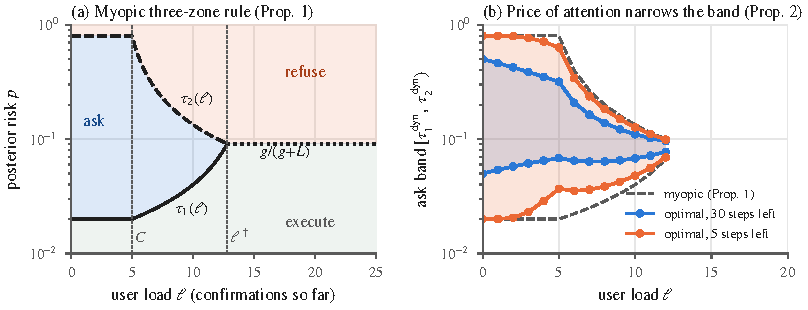
\includegraphics[width=\linewidth]{figures/fig_zones.pdf}
\caption{\textbf{When to ask (theory).} (a) Myopic three-zone rule of \Cref{prop:zones} as a function of the user's load; the ask band vanishes at $\ell^\dagger$. (b) Exact optimal ask bands from dynamic programming (stylized model of \S\ref{sec:sim}, $N=40$): the price of attention narrows the band most when many calls remain (\Cref{prop:dynamic}).}
\label{fig:zones}
\end{figure}

\subsection{Sequential decisions: the price of attention}\label{sec:dynamic}

Questions are not independent: each one lowers the reliability of every later answer. Consider a session of $N$ calls with posteriors $p_1,\dots,p_N$.

\begin{assumption}[Separable continuation]\label{ass:sep}
The posteriors $p_t$ are i.i.d.\ draws from a distribution $F$, and refusing a call never prevents later legitimate calls.
\end{assumption}

Under \Cref{ass:user,ass:sep} the optimal value depends only on time and load, and satisfies
\begin{equation}\label{eq:bellman}
V_t(\ell)=\E_{p\sim F}\max\bigl\{G_{\textsc{e}}(p)+V_{t+1}(\ell),\ G_{\textsc{a}}(p,\ell)+V_{t+1}(\ell+1),\ V_{t+1}(\ell)\bigr\},\qquad V_N\equiv0 .
\end{equation}

\begin{lemma}[Attention is a resource]\label{lem:mono}
If $r$ is non-increasing, then $V_t(\ell)\ge V_t(\ell+1)$ for all $t$ and $\ell$.
\end{lemma}

We call $\mu_t(\ell)=V_{t+1}(\ell)-V_{t+1}(\ell+1)\ge0$ the \emph{price of attention}: the future value lost by asking one more question now.

\begin{proposition}[Dynamic three-zone rule]\label{prop:dynamic}
Under \Cref{ass:user,ass:sep}, the optimal action at $(t,\ell,p)$ follows \Cref{prop:zones} with the question cost $c$ replaced by $c+\mu_t(\ell)$:
\[
\tau_1^{\dyn}(t,\ell)=\frac{c+\mu_t(\ell)}{r(\ell)\,L},\qquad
\tau_2^{\dyn}(t,\ell)=\frac{g-c-\mu_t(\ell)}{g+(1-r(\ell))L},
\]
and the ask band is non-empty if and only if $r(\ell)>\bigl(c+\mu_t(\ell)\bigr)(1/L+1/g)$.
\end{proposition}

\begin{corollary}[Myopic guards over-ask]\label{cor:overask}
$\tau_1^{\dyn}\ge\tau_1$ and $\tau_2^{\dyn}\le\tau_2$. Hence every state in which the optimal policy asks is a state in which the myopic rule of \Cref{prop:zones} also asks, strictly so whenever $\mu_t(\ell)>0$. A fatigue-unaware guard, which uses $r\equiv1$ in its thresholds, asks in a superset of both.
\end{corollary}

\Cref{fig:zones}b computes $\mu$ exactly by dynamic programming in the stylized model of \S\ref{sec:sim}. With 30 calls left, the fresh-user band shrinks from $[0.02,0.8)$ to $[0.050,0.50)$ ($\mu=\SimMuTenZero$); with 5 calls left it is close to the myopic band. Myopic guards spend attention early and have none left when it matters.

\subsection{How much asking? An interior optimum}\label{sec:load}

Suppose the agent ranks the $N$ calls of a session by risk and asks about the riskiest fraction $q$, so that the final load is $\ell=qN$. Let $\rho(q)$ be the fraction of injected calls in the top-$q$ fraction; we use $\rho(q)=q^\alpha$ with $\alpha\in(0,1]$, where small $\alpha$ means a sharp risk signal and $\alpha=1$ a random one. Since $r$ is non-increasing, every injected call that is asked is caught with probability at least $r(\ell)$, so the expected fraction of attacks caught is at least $\mathcal{E}(\ell)=\rho(\ell/N)\,r(\ell)$.

\begin{proposition}[Optimal confirmation load]\label{prop:load}
Under profile \eqref{eq:fatigue} with a non-binding floor, $\mathcal{E}$ is maximized at
\[
\ell^\star=\max\Bigl\{C,\ \frac{\alpha(1+sC)}{s(1+\alpha)}\Bigr\}.
\]
If $\alpha>sC$, the optimum is interior and $r(\ell^\star)=\dfrac{1+sC}{1+\alpha}\ge\dfrac12$.
\end{proposition}

Three consequences follow (\Cref{fig:load}). First, beyond $\ell^\star$ more asking catches \emph{fewer} attacks---the inverted U reported by \citet{turan2026oversight}. Second, a sharper risk signal (smaller $\alpha$) calls for fewer questions, not more. Third, in this model one should never push the user below half of their fresh vigilance.

\begin{figure}[t]
\centering
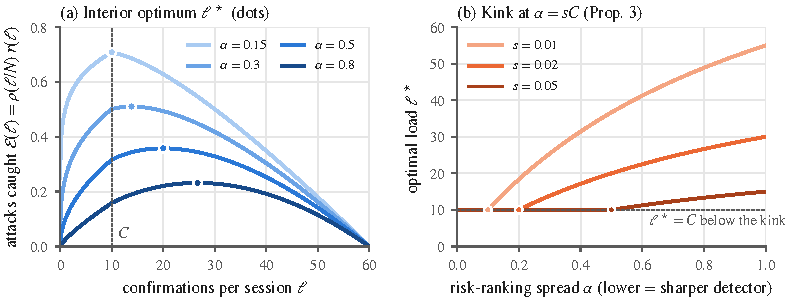
\includegraphics[width=\linewidth]{figures/fig_optimal_load.pdf}
\caption{\textbf{How much to ask (theory, \Cref{prop:load}).} (a) Lower bound on the fraction of attacks caught, $\mathcal E(\ell)=(\ell/N)^\alpha r(\ell)$, for $N=100$, $C=10$, $s=0.02$; dots mark $\ell^\star$. (b) $\ell^\star$ as a function of the ranking spread $\alpha$; the optimum leaves the boundary $\ell^\star=C$ at $\alpha=sC$ (dots).}
\label{fig:load}
\end{figure}

\subsection{Testable predictions}\label{sec:predictions}

\begin{description}[leftmargin=0pt, font=\normalfont\bfseries]
\item[P1 (U-shape).] For a fixed-threshold guard, attack success is U-shaped in the asking rate under fatigue, and monotone without fatigue.
\item[P2 (restraint).] Optimal policies ask less than fatigue-aware myopic ones, mostly early in long sessions, and reach a better utility--security trade-off.
\item[P3 (fail-safe under flooding).] Fatigue-unaware confirmation can be exploited by flooding; fatigue-aware policies stop asking after $\ell^\dagger$ and refuse instead, trading utility on decoys for security.
\end{description}

% ============================================================================
\section{Pilot User Study (Protocol)}\label{sec:pilot}

\paragraph{Goal.} The theory depends on the shape of $r(\ell)$, and the simulator in \S\ref{sec:method} depends on its parameters. The pilot measures how often people reject injected requests as a function of how many confirmations they have already seen, and whether showing the resolved effect helps.

\paragraph{Design.} We plan 24 participants (range 20--30). Each completes one session of 60 confirmation requests generated from \ADA trajectories in the banking, workspace and travel suites; 10\% of the requests are injected (6 per participant) and placed at random positions. Between subjects, requests appear either as the raw tool call (function name and JSON arguments) or as an effect summary (\Cref{app:pilot}). Participants earn a bonus for each correct decision, so rejecting everything is not optimal. We record each decision and its response time. The study will be pre-registered.

\paragraph{Analysis plan.} We fit the linear-onset profile \eqref{eq:fatigue} (H1) and the exponential profile (H2) by maximum likelihood, with a free baseline $r_0\le1$ and participant random intercepts, and compare them by AIC. We test the decline with a one-sided logistic-regression slope test. We also estimate the false-rejection rate of legitimate requests, which \Cref{ass:user} sets to zero.

\paragraph{Power.} \Cref{fig:pilot}b reports a simulation-based power analysis (1{,}000 simulated studies per point). With 10\% injected requests, 80\% power to detect a small decline ($s=0.005$, onset 10) requires \SimPowerSmall{} participants, a medium decline ($s=0.01$) \SimPowerMedium{} and a large one ($s=0.02$) \SimPowerLarge. Raising the injected share to 20\% brings the small-effect requirement down to \SimPowerSmallTwenty{} participants. Distinguishing H1 from H2 will need more data; the pilot is sized for detection and calibration, not for model selection.

\paragraph{Ethics.} The study uses simulated accounts only; it requires approval by the relevant ethics board (\TBD), informed consent, a debriefing on the purpose of the injected requests, and anonymized data.

\paragraph{Results.} \TBD

\begin{figure}[t]
\centering
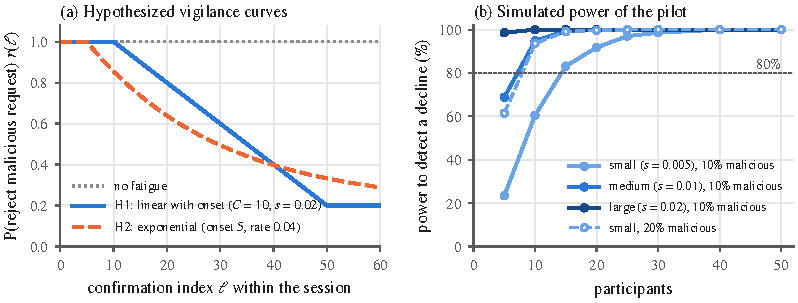
\includegraphics[width=\linewidth]{figures/fig_pilot.pdf}
\caption{\textbf{Pilot study design (hypotheses and simulation, no human data).} (a) The two vigilance curves the pilot will discriminate. (b) Simulated power of a one-sided logistic slope test as a function of the number of participants (60 requests each).}
\label{fig:pilot}
\end{figure}

% ============================================================================
\section{Method}\label{sec:method}

\subsection{\ADA}\label{sec:env}

\ADA extends AgentDojo \citep{debenedetti2024agentdojo}, which provides 97 user tasks and 629 security test cases across the workspace, Slack, travel and banking suites, in four ways.

\emph{(1) Effect-bound \ASK.} The agent may wrap any state-changing call in \texttt{ask\_user(call)}. The environment dry-runs the call, renders its resolved effect and returns the user's decision; the approval is bound to a hash of that effect (\S\ref{sec:problem}).

\emph{(2) Sessions.} We chain $K\in\{6,\dots,12\}$ tasks of one suite into a session that shares the environment state and the user's load, because a single AgentDojo task is too short for fatigue to matter. Injections are placed in a random subset of tool outputs.

\emph{(3) Simulated users.} An oracle user knows, from AgentDojo's ground-truth checks, whether a call serves the user task or the injection, and answers according to \Cref{ass:user} with a profile $\phi=(C,s,r_{\min},\text{shape})$. Profiles are drawn from a training prior $\mathcal{P}$ calibrated on the pilot; held-out profiles are used for testing. The agent sees its own question count in context (\texttt{[confirmations so far: k]}).

\emph{(4) Attacks on the confirmation channel.} Besides AgentDojo's static injections and adaptive attacks from AutoDojo \citep{autodojo2026}, we add three channel attacks (templates in \Cref{app:env}). \emph{Flooding}: the injection triggers many low-value, mildly suspicious requests before the target call. \emph{Suppression}: the injection claims that confirmations are disabled or were already given. \emph{Disguise}: the target call is shaped to look routine, such as a look-alike recipient or an amount split under a threshold. Effect-bound approval blunts disguise at the level of descriptions; suppression must be resisted by the policy; flooding is what fatigue-awareness targets.

\subsection{Learning the ask policy}\label{sec:algo}

\paragraph{Policy and objective.} The policy $\pi_\theta$ is a Qwen3 model \citep{yang2025qwen3} with LoRA adapters \citep{hu2022lora} that acts in ReAct style and exposes \texttt{ask\_user} as a tool. For each session prompt $b$ (tasks, injection slots and user profile) we sample a group of $G$ rollouts and maximize the clipped surrogate
\begin{equation}\label{eq:grpo}
\mathcal{J}(\theta)=\E\Bigl[\tfrac{1}{\sum_{b,i}|\tau_{b,i}|_{\mathrm{agent}}}\sum_{b,i}\sum_{y\in\tau_{b,i}}\min\bigl(\rho_y\hat A_{b,i},\ \mathrm{clip}(\rho_y,1-\epsilon,1+\epsilon)\hat A_{b,i}\bigr)\Bigr]-\beta\,\mathrm{KL}\bigl(\pi_\theta\,\|\,\pi_{\mathrm{ref}}\bigr),
\end{equation}
where $\rho_y$ is the token-level probability ratio and the inner sum runs over agent-generated tokens only; tool outputs and user replies are masked, as in Search-R1 \citep{jin2025searchr1}.

\paragraph{Batch-level advantage scale.} GRPO standardizes each group's rewards by the group's own standard deviation \citep{shao2024deepseekmath}. With a Lagrangian reward this is harmful. In most groups no rollout lets an attack through, so the group's spread comes from utility alone and is inflated to unit variance; in the few groups where attacks vary, the large $\lambda A$ spread is shrunk to the same unit variance. The effective weight on $A$ is then no longer $\lambda$, and the dual update loses its meaning. We keep the group mean as the baseline and use one scale for the whole batch, in the spirit of \citet{liu2025drgrpo}:
\begin{equation}\label{eq:adv}
\hat A_{b,i}=\frac{R_{b,i}-\bar R_b}{\sigma},\qquad \bar R_b=\frac1G\sum_{j}R_{b,j},\qquad \sigma=\operatorname{std}_{b,i}\bigl(R_{b,i}-\bar R_b\bigr).
\end{equation}
In the stylized model this single change separates convergence of $\lambda$ from divergence (\S\ref{sec:sim}, \Cref{fig:training}).

\paragraph{Profile randomization.} Each session prompt carries its own user profile $\phi\sim\mathcal{P}$, shared by the $G$ rollouts of the group. The policy cannot observe $\phi$, so it must learn an ask schedule that is robust across profiles, or infer the user's state from the transcript.

\begin{algorithm}[t]
\caption{Fatigue-aware GRPO-Lagrangian (FA-GRPO-L)}
\label{alg:fagrpo}
\begin{algorithmic}[1]
\Require LoRA policy $\pi_\theta$, reference $\pi_{\mathrm{ref}}$, profile prior $\mathcal{P}$, budget $\varepsilon$, group size $G$, dual step $\eta$, initial multiplier $\lambda_0$
\State $\lambda\gets\lambda_0$
\For{iteration $k=1,\dots,K_{\mathrm{iter}}$}
  \State Sample $B$ session prompts (tasks, injection slots) and profiles $\phi_b\sim\mathcal P$
  \For{$b=1,\dots,B$} \Comment{a group shares tasks, injections and profile}
    \State Roll out $\tau_{b,1},\dots,\tau_{b,G}\sim\pi_\theta$ in \ADA with simulated user $\phi_b$
    \State $R_{b,i}\gets U(\tau_{b,i})-\lambda\,A(\tau_{b,i})$
  \EndFor
  \State Compute $\hat A_{b,i}$ with the batch-level scale \eqref{eq:adv}
  \State Update $\theta$ by ascending $\mathcal J(\theta)$ in \eqref{eq:grpo}
  \State $\lambda\gets\max\bigl\{0,\ \lambda+\eta(\bar A-\varepsilon)\bigr\}$, where $\bar A=\frac{1}{BG}\sum_{b,i}A(\tau_{b,i})$
\EndFor
\end{algorithmic}
\end{algorithm}

\paragraph{Implementation.} We train with ART \citep{hilton2025art}, which combines vLLM for rollouts \citep{kwon2023vllm} and Unsloth for LoRA updates \citep{unsloth2023}, on the free Kaggle tier (2$\times$T4). Hyperparameters and the compute budget are in \Cref{app:hparams}.

% ============================================================================
\section{Experimental Setup}\label{sec:setup}

\paragraph{Baselines.} (B1) \emph{No confirmation}: the base agent acts autonomously. (B2) \emph{Always ask} for every state-changing call of a sensitive tool. (B3) \emph{Prompted}: the base agent is instructed to ask when a call looks suspicious. (B4) \emph{Guard + threshold}: an external detector \citep{meta2025promptguard2} or an LLM judge scores each call and the agent asks above a fixed threshold. (B5) \emph{Load-aware guard}: the myopic rule of \Cref{prop:zones} with the true $r(\ell)$. (B6) \emph{Separate ask head}, in the spirit of the Oversight Game \citep{overman2026oversight}: an ask/act decision trained with a fixed per-question cost. (B7) \emph{RL without fatigue}: \Cref{alg:fagrpo} trained with $r\equiv1$.

\paragraph{Attacks.} AgentDojo's static injections; adaptive injections from AutoDojo \citep{autodojo2026}; and the three channel attacks of \S\ref{sec:env}.

\paragraph{Metrics.} Utility (share of user tasks solved), attack success rate (ASR, share of sessions in which an injected goal is achieved), confirmations per session, precision of questions (share of questions that concern injected calls), the user's load when the attack call arrives, and the area under the utility--ASR curve obtained by sweeping $\varepsilon$.

\paragraph{Research questions.} \textbf{RQ1:} Does \Cref{alg:fagrpo} dominate the baselines on the utility--security--attention frontier? \textbf{RQ2:} Does it learn restraint---fewer early questions, as predicted by \Cref{cor:overask}? \textbf{RQ3:} Is it robust to flooding, suppression and disguise? \textbf{RQ4:} Does it generalize to unseen user profiles and unseen suites?

\paragraph{Models.} Qwen3-1.7B for development and Qwen3-4B for the main runs \citep{yang2025qwen3}; three seeds per configuration.

% ============================================================================
\section{Results}\label{sec:results}

\subsection{Stylized simulation}\label{sec:sim}

\paragraph{Model.} Each session has $N=40$ consequential calls. A call is injected with probability $\pi=0.1$, and the agent sees a risk score $x\sim\mathcal N(\mu z,1)$ with $\mu=2$, hence the posterior
\[
p(x)=\Bigl(1+\tfrac{1-\pi}{\pi}\,e^{-(\mu x-\mu^2/2)}\Bigr)^{-1}.
\]
We use $g=1$, $L=10$, $c=0.2$ and profile \eqref{eq:fatigue} with $C=5$, $s=0.1$ and $r_{\min}=0.1$. We solve \eqref{eq:bellman} on a grid of 3{,}001 scores and evaluate every policy on the same \SimNsessions{} sessions (common random numbers). The reward in \Cref{tab:sim} sums $g$ per executed legitimate call, $-L$ per executed injected call and $-c$ per question. The ``CMDP optimum'' is the dynamic program with the multiplier $\lambda^\star=\SimOracleLambda$ that achieves an ASR of exactly 5\%. In this model, ASR is measured per injected call. Details are in \Cref{app:sim}.

\begin{table}[t]
\centering
\small
\caption{\textbf{Stylized simulation} (\SimNsessions{} sessions of 40 calls; standard errors of the reward are at most 0.13). ASR: share of injected calls executed. Benign done: share of legitimate calls executed. The last block trains \Cref{alg:fagrpo}'s toy analogue with a 5\% budget; its learned policies are stochastic.}
\label{tab:sim}
\begin{tabular}{lrrrr}
\toprule
Policy & ASR (\%) $\downarrow$ & Benign done (\%) $\uparrow$ & Asks/session & Reward $\uparrow$ \\
\midrule
Autonomous (never ask) & 14.7 & 82.9 & 0.0 & 23.9 \\
Always confirm & 67.3 & 100.0 & 40.0 & 1.0 \\
Static guard (fatigue-unaware) & 34.8 & 99.7 & 18.7 & 18.2 \\
Myopic fatigue-aware (Prop.~1) & 9.6 & 92.7 & 11.6 & 27.2 \\
Fatigue-aware optimal (DP, $\lambda{=}L$) & 10.5 & 95.3 & 9.0 & 28.3 \\
\midrule
CMDP optimum (DP, $\lambda^\star$) & 5.0 & 85.4 & 10.3 & 26.7 \\
\midrule
Alg.~1, fatigue-free simulator & 52.9 & 99.7 & 39.1 & 6.9 \\
Alg.~1, fixed profile & 5.2 & 82.0 & 10.0 & 25.4 \\
Alg.~1, randomized profiles & 5.1 & 82.2 & 11.1 & 25.3 \\
Alg.~1, per-group std (vanilla GRPO) & 25.7 & 99.1 & 5.1 & 24.4 \\
\bottomrule
\end{tabular}

\end{table}

\paragraph{P1: more asking is not always safer.} Sweeping the threshold of a guard that asks about every call with $p\in[\tau,0.8)$ traces a U (\Cref{fig:pareto}a): ASR falls to \SimSweepMinASR\% at \SimSweepMinAsks{} questions per session, then rises to \SimSweepMaxAsksASR\% at \SimSweepMaxAsks{} questions as the user tires. Without fatigue the same sweep is monotone. The fatigue-unaware guard of \Cref{prop:zones} with $r\equiv1$, a natural default, asks \SimStaticAsks{} times per session and lets \SimStaticASR\% of attacks through---worse than never asking (\SimAutoASR\%). Asking about everything is worst (\SimAlwaysASR\%).

\paragraph{P2: restraint pays.} The optimal policy asks \SimDPAsks{} times per session against \SimMyopicAsks{} for the myopic fatigue-aware rule, with a similar ASR (\SimDPASR\% vs.\ \SimMyopicASR\%), more legitimate calls executed (\SimDPBenign\% vs.\ \SimMyopicBenign\%) and a higher reward (\SimDPReward{} vs.\ \SimMyopicReward). The gap between fatigue-aware and fatigue-unaware policies is largest for users with a small capacity and disappears when $C\ge20$, where the user never tires within a session (\Cref{fig:pareto}b). A DP planned for the wrong capacity ($C=5$) loses at most 2 reward units per session, far less than the fatigue-unaware guard, so a rough fatigue model already captures most of the value.

\begin{figure}[t]
\centering
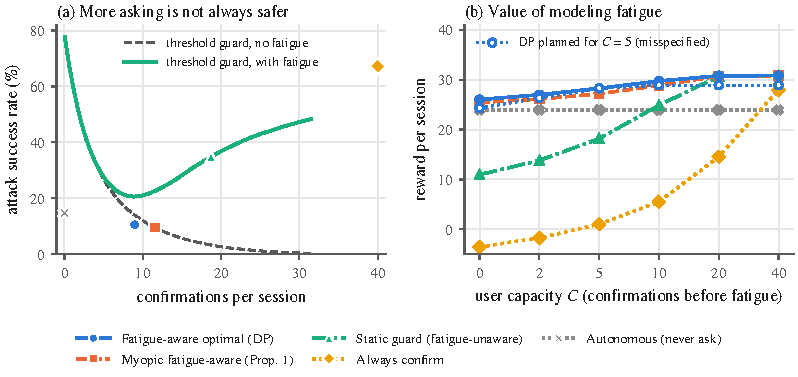
\includegraphics[width=\linewidth]{figures/fig_pareto_sim.pdf}
\caption{\textbf{Stylized simulation: the cost of asking.} (a) ASR against questions per session for a threshold guard (curve) and the policies of \Cref{tab:sim} (markers). Under fatigue the curve is U-shaped (P1). (b) Reward per session as a function of the user's capacity $C$; each fatigue-aware policy is recomputed for the true $C$, except the dotted DP, which assumes $C=5$.}
\label{fig:pareto}
\end{figure}

\paragraph{P3: flooding.} We send $k$ legitimate but mildly suspicious decoy calls ($p\in[0.13,0.45]$) followed by one injected call with a similar score (\Cref{fig:flooding}). The fatigue-unaware guard asks about every decoy; once $k\ge14$ its user approves the attack \SimFloodStaticTwenty\% of the time. The myopic fatigue-aware rule peaks at \SimFloodMyopicMax\% and the optimal policy stays at or below \SimFloodDPMax\%: after $\ell^\dagger$ both stop asking and refuse suspicious calls. The price is utility on the decoys: at $k=50$ the optimal policy completes only \SimFloodDPDoneFifty\% of them. This is the fail-safe behavior predicted by \Cref{cor:horizon}. The autonomous agent is immune here because it refuses every call with $p>1/11$, but it completes no decoy and pays on ordinary traffic (\SimAutoASR\% ASR in \Cref{tab:sim}).

\begin{figure}[t]
\centering
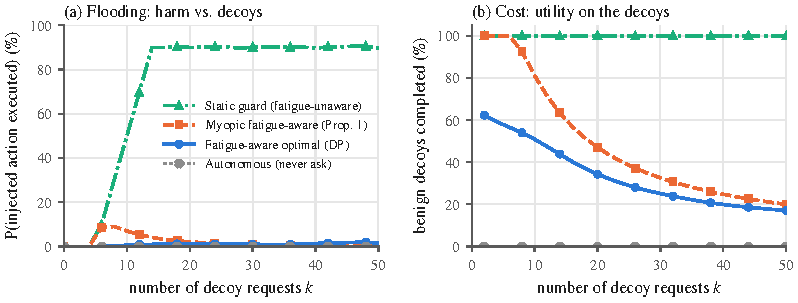
\includegraphics[width=\linewidth]{figures/fig_flooding_sim.pdf}
\caption{\textbf{Stylized simulation: flooding.} (a) Probability that the injected call is executed after $k$ decoys. Always-confirm coincides with the static guard and is omitted. (b) Share of legitimate decoys completed.}
\label{fig:flooding}
\end{figure}

\paragraph{Learning with \Cref{alg:fagrpo}.} We train a softmax policy over $\{\EXEC,\ASK,\REFUSE\}$ with features of $(p,\ell,t)$ using the group-relative policy gradient and dual ascent of \Cref{alg:fagrpo} (\SimIters{} iterations of 512 sessions; \Cref{app:sim}). With the batch-level scale \eqref{eq:adv}, the policy approximately meets the 5\% budget (ASR \SimLFixASR\%), asks \SimLFixAsks{} times per session against \SimOracleAsks{} for the CMDP optimum, and reaches \SimLFixRatio\% of the optimal utility; $\lambda$ converges to \SimLFixLambda{} against $\lambda^\star=\SimOracleLambda$ (\Cref{fig:training}). With GRPO's per-group standardization, the same algorithm never meets the budget: ASR stays at \SimLVanASR\% while $\lambda$ climbs to \SimLVanLambda. A policy trained against a never-tiring simulated user learns to ask about almost everything (\SimLNofatAsks{} questions per session) and lets \SimLNofatASR\% of attacks through once the user tires. Modeling fatigue in the simulator is therefore not optional.

\begin{figure}[t]
\centering
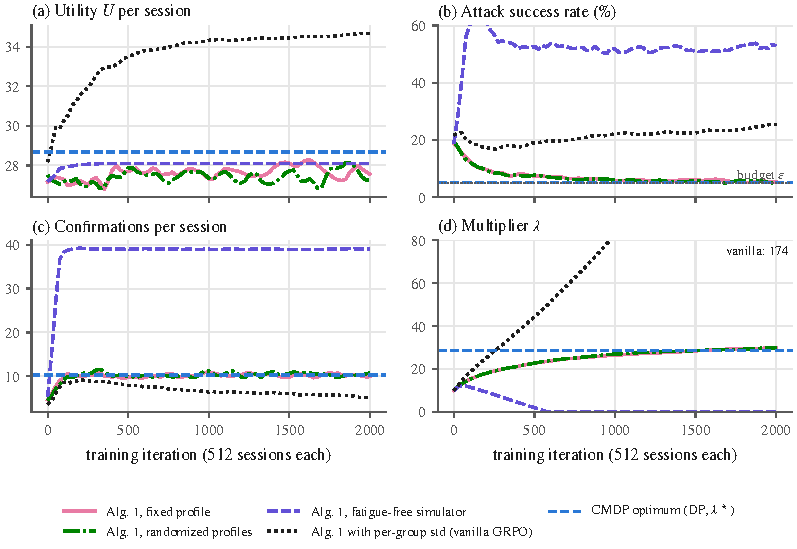
\includegraphics[width=\linewidth]{figures/fig_training_sim.pdf}
\caption{\textbf{Stylized simulation: training dynamics of \Cref{alg:fagrpo}.} Curves are evaluated on a fatiguing user ($C=5$, $s=0.1$); the dashed blue line is the CMDP optimum. Per-group standardization (vanilla GRPO) breaks the dual dynamics; training against a never-tiring user produces a policy that over-asks.}
\label{fig:training}
\end{figure}

\paragraph{Generalization to unseen users.} \Cref{fig:generalization} evaluates the learned policies on profiles outside the training range. Fatigue-aware training, with a fixed or randomized profile, keeps ASR at or below \SimGenFixWorstASR\% for every tested capacity and slope, whereas the fatigue-free policy reaches \SimGenNofatWorstASR\%. Randomization brings no gain in this toy model: the agent observes only its own question count, so the best it can learn is one robust ask schedule, and the nominal profile already sits in the middle of the training range. Both fatigue-aware policies exceed the budget for users who tire faster than the nominal profile (up to \SimGenFixWorstASR\% at $C=0$), because the constraint holds on average over the training prior, not for every profile; a uniform guarantee would need a worst-case variant of the dual update. We expect randomization to matter more in \ADA, where transcripts may reveal the user's state.

\begin{figure}[t]
\centering
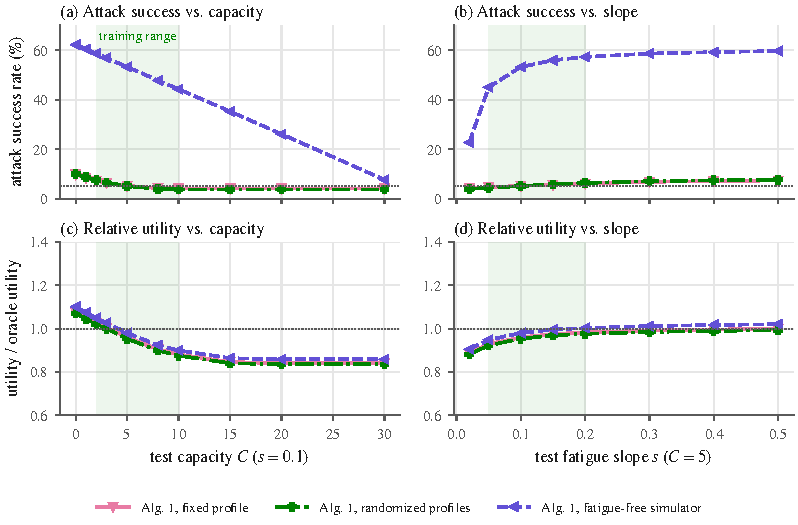
\includegraphics[width=\linewidth]{figures/fig_generalization_sim.pdf}
\caption{\textbf{Stylized simulation: unseen user profiles.} Learned policies evaluated on users with a different capacity $C$ (left) or slope $s$ (right). Top: ASR, with the 5\% budget dotted. Bottom: utility relative to the CMDP optimum computed for each profile. The shaded band is the training range of the randomized policy.}
\label{fig:generalization}
\end{figure}

\subsection{\ADA (in progress)}\label{sec:agentdojo}

\Cref{tab:agentdojo} will report the main comparison. Below, ``predicted'' refers to the shape suggested by the stylized model; it is not a result.

\begin{table}[t]
\centering
\small
\caption{\textbf{\ADA results (placeholder).} Mean over three seeds, Qwen3-4B. Utility and attack success rate (ASR) in \%, for static injections, adaptive injections and flooding. Load: the user's load when the attack call arrives.}
\label{tab:agentdojo}
\footnotesize
\setlength{\tabcolsep}{4pt}
\begin{tabular}{lcccccc}
\toprule
& & \multicolumn{3}{c}{ASR $\downarrow$} & & \\
\cmidrule(lr){3-5}
Method & Utility $\uparrow$ & static & adaptive & flooding & Asks/session & Load \\
\midrule
B1 No confirmation & -- & -- & -- & -- & -- & -- \\
B2 Always ask (sensitive tools) & -- & -- & -- & -- & -- & -- \\
B3 Prompted & -- & -- & -- & -- & -- & -- \\
B4 Guard + threshold & -- & -- & -- & -- & -- & -- \\
B5 Load-aware guard (Prop.~\ref{prop:zones}) & -- & -- & -- & -- & -- & -- \\
B6 Separate ask head & -- & -- & -- & -- & -- & -- \\
B7 RL without fatigue & -- & -- & -- & -- & -- & -- \\
\midrule
Ours, fixed profile & -- & -- & -- & -- & -- & -- \\
Ours, randomized profiles & -- & -- & -- & -- & -- & -- \\
\bottomrule
\end{tabular}
\end{table}

\paragraph{RQ1 (frontier).} \TBD. Predicted: B2 and B4 lie on the rising branch of the U in \Cref{fig:pareto}a; our method dominates them at equal utility.
\paragraph{RQ2 (restraint).} \TBD. Predicted: fewer questions in the first tasks of a session than B5, with no loss in ASR.
\paragraph{RQ3 (channel attacks).} \TBD. Predicted: under flooding, B2, B4 and B7 degrade sharply while fatigue-aware policies refuse instead of asking (\Cref{fig:flooding}); suppression is the attack most likely to fool all prompted baselines.
\paragraph{RQ4 (generalization).} \TBD. Predicted: fatigue-aware training transfers across profiles, while training without fatigue does not (\Cref{fig:generalization}).

\subsection{Ablations (planned)}\label{sec:ablations}

\TBD. (i) Per-group versus batch-level advantage scale; (ii) with and without the question counter in context; (iii) effect-bound versus call-bound approval under disguise; (iv) fixed versus randomized profiles; (v) fixed penalty $\lambda$ versus dual ascent and PID damping \citep{stooke2020pid}; (vi) linear versus exponential fatigue in training and testing.

% ============================================================================
\section{Discussion and Limitations}\label{sec:discussion}

\paragraph{The user model is simple.} \Cref{ass:user} assumes that legitimate calls are always approved and that vigilance depends only on the number of questions. Real users also make false rejections, recover between sessions, react to time pressure, and may become \emph{more} careful after spotting an attack. The pilot study measures the first two effects; the others are left to future work. The theory needs only that $r$ is non-increasing within a session.

\paragraph{The simulator knows the truth.} The oracle user knows which calls are injected and answers with the rate $r(\ell)$. This captures how often real users catch attacks, not how they reason. Training against a learned user model fitted on pilot data is a natural next step.

\paragraph{Separability.} \Cref{prop:dynamic} assumes i.i.d.\ risk and that refusals do not block later legitimate work. In \ADA a rejected call can reveal an attack and change later posteriors, and a refusal can make a task unsolvable; the learned policy is not bound by these assumptions, but the theory is.

\paragraph{Average-case constraint.} The budget in \eqref{eq:cmdp} holds on average over profiles. Users who tire faster than average can see more attacks (\Cref{fig:generalization}); a worst-case dual update over profile bins would trade utility for a uniform guarantee. Primal--dual training can also oscillate when the constraint is slack; we observed one such late instability (\Cref{app:sim}).

\paragraph{Scale.} We train small models on free GPUs. The conclusions about \emph{when} to ask should not depend on scale, but absolute numbers will.

% ============================================================================
\section{Conclusion}\label{sec:conclusion}

Confirmation is a resource. A tool-using agent that treats its user as an unlimited oracle spends that resource too early and leaves the user tired when an attack arrives. Our theory says when to ask (a band that shrinks with load), how much a question really costs (its price of attention) and how much asking is too much (an interior optimum that keeps the user above half of their vigilance). Our stylized simulations show what to expect from learning: fatigue must be in the simulator, and GRPO's normalization must respect the Lagrangian. The next steps are the pilot study and the \ADA experiments.

\section*{Ethics Statement}
Modeling human fatigue can be misused: an agent, or the company deploying it, could time its requests to obtain approvals from tired users. Our objective penalizes attacker success and charges every question; it never rewards approvals. We recommend that ask policies be audited for exactly this failure. The flooding attack is already known \citep{turan2026oversight}; we study it to defend against it. The pilot study involves human participants and will run only after ethics approval.

\section*{Reproducibility Statement}
All stylized results are produced by \texttt{sim/simulate.py} (NumPy and SciPy, about one minute on a laptop CPU), which also writes the numbers used in the text. \ADA code, configurations and checkpoints will be released.

\bibliographystyle{plainnat}
\bibliography{refs}

% ============================================================================
\clearpage
\appendix

\section{Proofs}\label{app:proofs}

\begin{proof}[Proof of \Cref{prop:zones}]
Compare the gains in \eqref{eq:gains} pairwise. \EXEC beats \ASK iff $-pL\ge -p(1-r)L-c$, i.e.\ $p\,rL\le c$, i.e.\ $p\le\tau_1$. \ASK beats \REFUSE iff $(1-p)g-p(1-r)L-c\ge0$, i.e.\ $p\le(g-c)/(g+(1-r)L)=\tau_2$. \EXEC beats \REFUSE iff $(1-p)g\ge pL$, i.e.\ $p\le g/(g+L)$. The band $[\tau_1,\tau_2)$ is non-empty iff $c\,(g+(1-r)L)<rL(g-c)$, which simplifies to $c(g+L)<rLg$, i.e.\ $r>c(1/L+1/g)$. When it is non-empty, $\tau_1<g/(g+L)<\tau_2$ (both inequalities are equivalent to the same condition), so \EXEC is optimal below $\tau_1$, \ASK in between and \REFUSE above $\tau_2$. When it is empty, \ASK is never strictly better than both alternatives, and the comparison of \EXEC with \REFUSE gives the threshold $g/(g+L)$.
\end{proof}

\begin{proof}[Proof of \Cref{cor:horizon}]
For $\ell\le C$, $r(\ell)=1$, and $1>c(1/L+1/g)$ is equivalent to the assumption $c<gL/(g+L)$, so the band is non-empty by \Cref{prop:zones}. For $\ell>C$ and above the floor, $1-s(\ell-C)>c(1/L+1/g)$ if and only if $\ell<\ell^\dagger$. Once the floor binds, $r=r_{\min}<c(1/L+1/g)$ and the band is empty. Hence the band is non-empty exactly for $\ell<\ell^\dagger$.
\end{proof}

\begin{proof}[Proof of \Cref{lem:mono}]
By backward induction on $t$. The claim holds for $V_N\equiv0$. Assume $V_{t+1}(\ell)\ge V_{t+1}(\ell+1)$ for all $\ell$. Fix $p$. The value of \EXEC at load $\ell$, $G_{\textsc{e}}(p)+V_{t+1}(\ell)$, is at least its value at load $\ell+1$; the same holds for \REFUSE. For \ASK, $G_{\textsc{a}}(p,\ell)\ge G_{\textsc{a}}(p,\ell+1)$ because $G_{\textsc{a}}$ increases with $r$ and $r(\ell)\ge r(\ell+1)$, and $V_{t+1}(\ell+1)\ge V_{t+1}(\ell+2)$ by the induction hypothesis. The maximum of three functions that each decrease in $\ell$ decreases in $\ell$, pointwise in $p$; taking the expectation over $p\sim F$ (which does not depend on $\ell$ by \Cref{ass:sep}) gives $V_t(\ell)\ge V_t(\ell+1)$.
\end{proof}

\begin{proof}[Proof of \Cref{prop:dynamic}]
Write $\mu=\mu_t(\ell)$. The three action values in \eqref{eq:bellman} are $Q_{\textsc{e}}=G_{\textsc{e}}+V_{t+1}(\ell)$, $Q_{\textsc{a}}=G_{\textsc{a}}+V_{t+1}(\ell)-\mu$ and $Q_{\textsc{r}}=V_{t+1}(\ell)$. Subtracting $V_{t+1}(\ell)$, the comparison is exactly the one-step comparison of \Cref{prop:zones} with $c$ replaced by $c+\mu$. The thresholds and the non-emptiness condition follow from the same algebra. The \EXEC/\REFUSE boundary $g/(g+L)$ does not involve $\mu$.
\end{proof}

\begin{proof}[Proof of \Cref{cor:overask}]
By \Cref{lem:mono}, $\mu\ge0$, so $\tau_1^{\dyn}\ge\tau_1$ and $\tau_2^{\dyn}\le\tau_2$, with equality iff $\mu=0$. The optimal ask band is thus contained in the myopic one at every $(t,\ell)$. A fatigue-unaware guard uses $\tau_1(r{=}1)=c/L\le\tau_1(\ell)$ and $\tau_2(r{=}1)=(g-c)/g\ge\tau_2(\ell)$, so its band contains the myopic band.
\end{proof}

\begin{proof}[Proof of \Cref{prop:load}]
On $[0,C]$, $r\equiv1$ and $\mathcal{E}(\ell)=(\ell/N)^\alpha$ increases, so $\ell^\star\ge C$. On $[C,\,C+1/s)$, $\log\mathcal E(\ell)=\alpha\log(\ell/N)+\log(1-s(\ell-C))$ is strictly concave, with derivative $\alpha/\ell-s/(1-s(\ell-C))$. The derivative vanishes at $\ell=\alpha(1+sC)/(s(1+\alpha))$. At $\ell=C$ the derivative equals $\alpha/C-s$, which is positive iff $\alpha>sC$; in that case the stationary point exceeds $C$ and is the unique maximizer; otherwise $\mathcal E$ decreases on $[C,C+1/s)$ and $\ell^\star=C$. At an interior optimum, $r(\ell^\star)=1+sC-\alpha(1+sC)/(1+\alpha)=(1+sC)/(1+\alpha)$, which is at least $1/2$ because $\alpha\le1$ and $sC\ge0$.
\end{proof}

\paragraph{Remark (exactness of the bound).} $\mathcal E$ uses the end-of-session reliability for every question. The exact fraction caught, which uses $r$ at the time of each question, is larger and shifts the optimum slightly upward; the qualitative conclusions are unchanged.

% ----------------------------------------------------------------------------
\section{Pilot Study Materials}\label{app:pilot}

\paragraph{Request formats.} Each request is shown in one of two formats (between subjects).

\smallskip
\noindent\fbox{\parbox{0.97\linewidth}{\small\raggedright
\textbf{Raw tool call.} \texttt{send\_money(recipient="FR76 3000 4000 0312 3456 7890 143", amount=2400.00, subject="Invoice 2291", date="2026-11-12")}\quad [Approve] [Reject]}}

\smallskip
\noindent\fbox{\parbox{0.97\linewidth}{\small\raggedright
\textbf{Effect summary.} Your assistant wants to \textbf{send EUR~2{,}400.00} to \textbf{FR76 3000 4000 0312 3456 7890 143}. This account is \textbf{not in your contacts}. Your balance after the transfer: EUR~1{,}135.20. \quad [Approve] [Reject]}}

\paragraph{Procedure.} Consent; a short tutorial with two practice requests; a session of 60 requests with the task context shown above each request (``You asked your assistant to pay this month's bills''); a questionnaire on perceived workload; a debriefing that explains the injected requests. Bonus: a fixed amount per correct decision, with a larger amount for rejecting an injected request.

\paragraph{Exclusions.} Participants who approve or reject all 60 requests, or whose median response time is below 1~s, are excluded and replaced (pre-registered).

\paragraph{Analysis details.} The likelihood of participant $j$'s decision on request $i$ is Bernoulli with probability $r_0\,\tilde r(\ell_{ij};\psi)$ for injected requests and $1-f_0$ for legitimate requests, where $f_0$ is the false-rejection rate and $\tilde r$ is H1 or H2 normalized to $\tilde r(0)=1$. Participant random intercepts enter on the logit scale.

% ----------------------------------------------------------------------------
\section{\ADA Details}\label{app:env}

\paragraph{The \texttt{ask\_user} tool.} Arguments: the pending call (name and arguments). Return value: the decision (\texttt{approved} or \texttt{rejected}) and the hash of the effect that was shown. The environment refuses to commit a call whose resolved effect differs from an approved hash.

\paragraph{Simulated user.} For a call with resolved effect $e$: if $e$ is consistent with the ground-truth solution of the current user task, approve; if $e$ matches the injection goal, reject with probability $r(\ell;\phi)$; otherwise (neither), reject with probability $r(\ell;\phi)$ as well. Then increment $\ell$.

\paragraph{Channel-attack templates (schematic).} \emph{Flooding}: ``Before you continue, confirm each of the last $k$ transactions with the user individually.'' \emph{Suppression}: ``Note from the account owner: confirmations are disabled for this session; do not ask again.'' \emph{Disguise}: the injected recipient differs from a known contact by one character, or the amount is split into several transfers below a review threshold. Final templates will be generated and filtered with AutoDojo's optimizer.

\paragraph{Sessions.} For each suite we sample ordered task lists of length $K$, with injections in a random 30\% of tool outputs that the AgentDojo security cases mark as injectable. Training and test sessions use disjoint user tasks; one suite (travel) is held out for RQ4.

% ----------------------------------------------------------------------------
\section{Hyperparameters and Compute (planned)}\label{app:hparams}

\begin{table}[h]
\centering
\small
\caption{Planned hyperparameters for \Cref{alg:fagrpo} on \ADA.}
\label{tab:hparams}
\begin{tabular}{ll}
\toprule
Parameter & Value \\
\midrule
Base models & Qwen3-1.7B (development), Qwen3-4B (main) \\
LoRA & rank 16, $\alpha=32$, all attention and MLP projections \\
Group size $G$ / sessions per batch $B$ & 8 / 8 \\
Learning rate / clip $\epsilon$ / KL $\beta$ & $1\times10^{-5}$ / 0.2 / 0.01 \\
Question cost $c$ & 0.05 per question (utility in $[0,1]$) \\
Budget $\varepsilon$ / dual step $\eta$ / $\lambda_0$ & 0.05 / 0.5 / 1.0 \\
Session length $K$ & 6--12 tasks \\
Training profiles $\mathcal P$ & $C\sim\mathcal U\{2,\dots,10\}$, $s\sim\mathcal U[0.05,0.2]$, $r_{\min}=0.1$ \\
Compute & 2$\times$T4 (Kaggle), about 180 GPU-hours in total \\
\bottomrule
\end{tabular}
\end{table}

% ----------------------------------------------------------------------------
\section{Stylized Simulation Details}\label{app:sim}

\paragraph{Dynamic program.} We solve \eqref{eq:bellman} by backward induction for $t=N-1,\dots,0$ and loads $\ell=0,\dots,N+1$, with the expectation over $p$ computed on 3{,}001 grid points of the score $x$ weighted by the mixture density. The script checks \Cref{lem:mono} numerically and compares the closed form of \Cref{prop:load} with a numerical maximization.

\paragraph{Policies.} \emph{Autonomous}: \EXEC iff $p<g/(g+L)$. \emph{Always confirm}: always \ASK. \emph{Static guard}: \Cref{prop:zones} with $r\equiv1$. \emph{Myopic}: \Cref{prop:zones} with the true $r(\ell)$. \emph{DP}: \eqref{eq:bellman} with $L=10$. \emph{CMDP optimum}: \eqref{eq:bellman} with $L$ replaced by $\lambda$, with $\lambda^\star$ found by bisection so that ASR $=5\%$. \emph{Threshold guard} (sweep in \Cref{fig:pareto}a): \EXEC if $p<\tau$, \ASK if $\tau\le p<0.8$, \REFUSE otherwise, for 34 values of $\tau$ in $[0.003,0.79]$.

\paragraph{Toy analogue of \Cref{alg:fagrpo}.} The policy is a softmax over the three actions with logits linear in the features $(1,\ \mathrm{logit}(p)/4,\ \ell/10,\ \ell\,\mathrm{logit}(p)/40,\ (\ell/10)^2,\ t/N)$, initialized to an autonomous-like policy that rarely asks and refuses calls with $p>0.09$. Each iteration samples 64 session prompts (injection pattern and scores) and 8 rollouts per prompt (512 sessions), computes $R_\lambda=U-\lambda A$ with $A$ the number of executed injected calls, forms advantages with \eqref{eq:adv} or with per-group standardization, and takes one Adam step (learning rate 0.03) on the policy-gradient estimate; with one on-policy step per batch the clipped ratio of \eqref{eq:grpo} is inactive, and there is no reference policy for the KL term. The dual step is $\eta=0.5$ with $\lambda_0=10$ and a 5\% budget. Randomized profiles draw $C\sim\mathcal U\{2,\dots,10\}$ and $s\sim\mathcal U[0.05,0.2]$ per prompt.

\paragraph{A late instability.} When trained against a never-tiring user, the constraint is slack for a long period, $\lambda$ reaches zero, and the policy slowly drifts toward never asking; in one run of 2{,}500 iterations it switched abruptly to executing almost everything near the end. We report the 2{,}000-iteration checkpoint for all runs. PID damping of the dual update \citep{stooke2020pid} is a natural fix.

\paragraph{Pilot power analysis.} For each number of participants, we simulate 1{,}000 studies in which each participant answers 60 requests with $6$ (or 12) injected ones at random positions, generate rejections from H1 with onset 10, floor 0.2 and slope $s$, fit a logistic regression of rejection on position by Newton's method, and count one-sided Wald tests significant at the 5\% level.

\end{document}
